% kmc_step.png: one step of first-order KMC, the twelve jumps and the selection of one of them. The probabilities are an example.
% Make it in this folder with, for any scratch folder T:
%   pdflatex -output-directory=T fig_kmc_step.tex
%   python3 pdf_to_png.py T/fig_kmc_step.pdf ../kmc_step.png
\documentclass[11pt,tikz,border=1.5pt]{standalone}
% Shared preamble of all figures. Every fig_*.tex is compiled on its own, see the comment at its top; the fonts are those of the matplotlib
% style xzc_sans (amsmath, amssymb, amsfonts, sfmath), so that line drawings and data plots look the same.
\usepackage{amsmath,amssymb,amsfonts}
\usepackage{sfmath}
\renewcommand{\familydefault}{\sfdefault}
\usepackage{graphicx}
\usetikzlibrary{arrows.meta,calc,positioning,decorations.pathreplacing,backgrounds,shapes.geometric}
% species: Al gray, Mg orange, Zn blue; red marks the vacancy and the jumping atom
\definecolor{cAl}{HTML}{B8BCC2}
\definecolor{cMg}{HTML}{E08A2E}
\definecolor{cZn}{HTML}{3F78B5}
\definecolor{cOne}{HTML}{C8423B}
\definecolor{cTwo}{HTML}{3F78B5}
\definecolor{cThree}{HTML}{3E9B5C}
\definecolor{cFour}{HTML}{E0A21B}
\definecolor{cGray}{HTML}{7E858F}
\definecolor{cDark}{HTML}{2B2B2B}
\newcommand{\panel}[1]{\textbf{(#1)}}
\newcommand{\DM}{D_{\mathrm{MEP}}}
\newcommand{\KI}{K_{\mathrm{I}}}
\newcommand{\KF}{K_{\mathrm{F}}}
\newcommand{\dE}{\Delta E}
\newcommand{\Ea}{\Delta E_{\mathrm{a}}}
\newcommand{\ea}{\Delta e_{\mathrm{a}}}
\newcommand{\Ebind}{E_{\mathrm{bind}}^{\mathrm{site}}}
% a ball with a soft highlight, like the rendered spheres
\makeatletter
\pgfdeclareradialshading[tikz@ball]{softball}{\pgfpoint{-9bp}{9bp}}{%
  color(0bp)=(tikz@ball!22!white); color(6bp)=(tikz@ball!62!white); color(13bp)=(tikz@ball!96!white);
  color(20bp)=(tikz@ball!92!black); color(27bp)=(tikz@ball!74!black); color(50bp)=(tikz@ball!55!black)}
\makeatother
\tikzset{
  every picture/.append style={line cap=round, line join=round},
  every node/.append style={font=\small},
  img/.style={inner sep=0pt, anchor=south west},
  lab/.style={font=\normalsize, inner sep=1pt, anchor=north west},
  above lab/.style={font=\normalsize, inner sep=1pt, anchor=south west},
  capt/.style={align=center, anchor=north},
  atom/.style={circle, ball color=#1, shading=softball, minimum size=12pt, inner sep=0pt},
  atom/.default=cAl,
  vac/.style={circle, draw=cOne, line width=1.1pt, fill=white, minimum size=11.5pt, inner sep=0pt},
  arr/.style={-{Stealth[length=5pt]}, line width=0.8pt},
  dbl/.style={{Stealth[length=4pt]}-{Stealth[length=4pt]}, line width=0.8pt},
  jump/.style={arr, cOne, line width=1.2pt},
  block/.style={-{Triangle[length=8pt, width=13pt]}, line width=5pt, cTwo!38},
  cell axis/.style={-{Triangle[length=6pt, width=5.5pt]}, line width=1.2pt, black},
  dir/.style={fill=white, fill opacity=0.75, text opacity=1, font=\footnotesize, inner sep=1.5pt},
}
\graphicspath{{img/}}
% data plots are included at one scale: \plot{name}{x}{y}{file}
\newcommand{\plotscale}{0.6}
\newcommand{\plot}[4]{\node[img] (#1) at (#2,#3) {\includegraphics[scale=\plotscale]{#4}};}
\newcommand{\plotlabel}[2]{\node[above lab] at ($(#1.north west)+(-0.05,0.02)$) {\panel{#2}};}
% legend of the species, first entry at (#1,#2): Al, Mg, Zn (and the vacancy)
\tikzset{leg/.style={anchor=base west, inner sep=2pt, yshift=-3.2pt}}
\newcommand{\specieslegend}[2]{%
  \foreach \lx/\lc/\lt in {0/cAl/Al, 1.2/cMg/Mg, 2.4/cZn/Zn} {
    \node[atom=\lc, minimum size=10pt] at ({#1+\lx},#2) {}; \node[leg] at ({#1+\lx+0.2},#2) {\lt};}}
\newcommand{\vacancylegend}[2]{\node[vac, minimum size=9.5pt] at (#1,#2) {}; \node[leg] at ({#1+0.2},#2) {vacancy};}

% number of the jump / its probability / end of its segment / atom on the site / color of the arrow
\newcommand{\jumps}{1/0.02/0.02/cAl/black!70, 2/0.05/0.07/cAl/black!70, 3/0.02/0.09/cAl/black!70, 4/0.30/0.39/cZn/black!70,
  5/0.02/0.41/cAl/black!70, 6/0.08/0.49/cMg/black!70, 7/0.02/0.51/cAl/black!70, 8/0.22/0.73/cMg/cOne,
  9/0.03/0.76/cAl/black!70, 10/0.15/0.91/cZn/black!70, 11/0.04/0.95/cAl/black!70, 12/0.05/1.00/cAl/black!70}
\begin{document}
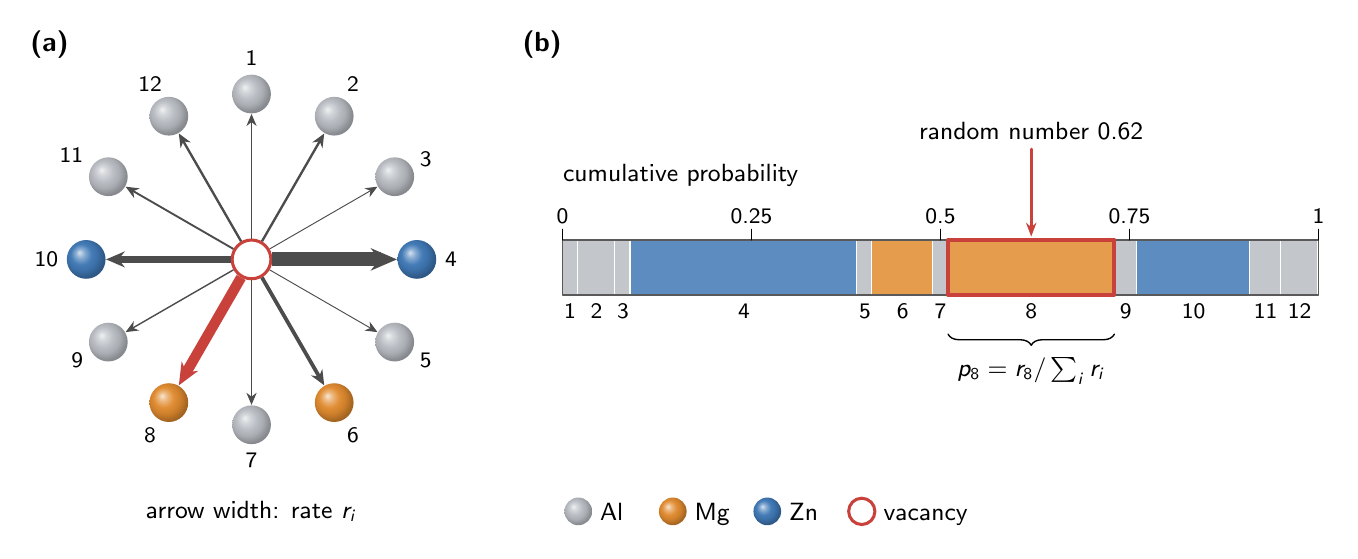
\begin{tikzpicture}
  % ---------------- (a) the twelve jumps, drawn in a ring; the width of an arrow is proportional to the rate ----------------
  \begin{scope}
    \node[vac, minimum size=14pt] (v) at (0,0) {};
    \foreach \num/\prob/\stop/\atom/\acol in \jumps {
      \pgfmathsetmacro{\ang}{90 - (\num-1)*30}
      \pgfmathsetmacro{\opp}{\ang + 180}
      \pgfmathsetmacro{\lw}{17*\prob}
      \pgfmathsetmacro{\headl}{4.0 + 18*\prob}
      \pgfmathsetmacro{\headw}{0.85*\headl}
      \node[atom=\atom, minimum size=14pt] (n\num) at (\ang:2.1cm) {};
      \draw[-{Stealth[length=\headl pt, width=\headw pt]}, line width=\lw pt, \acol, line cap=butt] (v) -- (n\num);
      \node[font=\footnotesize, anchor=\opp, inner sep=2pt] at (\ang:2.38cm) {\num};
    }
    \node at (0,-3.2) {arrow width: rate $r_i$};
  \end{scope}
  % ---------------- (b) the probabilities, laid end to end, and a random number ----------------
  \begin{scope}[shift={(3.95,-0.45)}]
    \def\W{9.6}
    \foreach \num/\prob/\stop/\atom/\acol in \jumps {
      \fill[\atom!85] ({(\stop-\prob)*\W},0) rectangle (\stop*\W,0.7);
      \draw[white, line width=0.8pt] (\stop*\W,0) -- (\stop*\W,0.7);
      \node[font=\footnotesize, anchor=north, inner sep=3pt] at ({(\stop-\prob/2)*\W},0) {\num};
    }
    \draw[black!65, line width=0.6pt] (0,0) rectangle (\W,0.7);
    \draw[cOne, line width=1.4pt] (0.51*\W,0) rectangle (0.73*\W,0.7);
    \foreach \t in {0, 0.25, 0.5, 0.75, 1} {
      \draw[line width=0.6pt] (\t*\W,0.7) -- ++(0,0.13) node[font=\footnotesize, anchor=south, inner sep=2pt] {\t};}
    \draw[jump] (0.62*\W,1.85) -- (0.62*\W,0.74);
    \node[anchor=south] at (0.62*\W,1.85) {random number 0.62};
    \node[anchor=south west, inner xsep=0pt] at (0,1.25) {cumulative probability};
    \draw[decorate, decoration={brace, mirror, amplitude=4pt}, line width=0.5pt]
         (0.51*\W,-0.50) -- (0.73*\W,-0.50) node[midway, below=5pt] {$p_8 = r_8/\sum_i r_i$};
  \end{scope}
  \specieslegend{4.15}{-3.2}
  \vacancylegend{7.75}{-3.2}
  \node[lab] at (-2.85,2.95) {\panel{a}};
  \node[lab] at (3.40,2.95) {\panel{b}};
\end{tikzpicture}
\end{document}
